
\documentclass[11pt]{exam} % https://www.ctan.org/pkg/exam?lang=en

\usepackage[lmargin=1.in,rmargin=1.in,tmargin=1.in,bmargin=1in]{geometry}
\usepackage{setspace}
\usepackage[pdftex]{graphicx}
\usepackage{titling}
\usepackage[
	pdfauthor={Brian Weinstein},
	pdftitle={Homework 1},
	bookmarks=true,
	colorlinks=true,
	linkcolor=blue,
	urlcolor=blue,
	citecolor=blue,
	pdftex,
	linktocpage=true
	]{hyperref}
\usepackage[textsize=tiny]{todonotes}
\usepackage{float}
\setlength\parindent{0pt}
\usepackage{lipsum}


\qformat{\textbf{Problem \thequestion: \thequestiontitle}\quad \hfill}


\pagestyle{headandfoot}
\runningheadrule
\firstpageheader{}{}{}
\runningheader{\theauthor}{\thetitle}{\thedate}
\firstpagefooter{}{\thepage}{}
\runningfooter{}{\thepage}{}


\usepackage{xcolor}
\usepackage{adjustbox}
\usepackage{verbatim}
\definecolor{shadecolor}{rgb}{.9, .9, .9}

\newenvironment{code}%
   {\par\noindent\adjustbox{margin=1ex,bgcolor=shadecolor,margin=0ex \medskipamount}\bgroup\minipage\linewidth\verbatim}%
   {\endverbatim\endminipage\egroup}

\newenvironment{codeSmall}%
   {\par\noindent\adjustbox{margin=1ex,bgcolor=shadecolor,margin=0ex \medskipamount}\bgroup\minipage\linewidth\verbatim\footnotesize}%
   {\endverbatim\endminipage\egroup}

\newcommand{\ramsey}{\href{http://www.statisticalsleuth.com/}{Ramsey }}


\begin{document}


\title{STAT S4201 001, Homework 1}
\author{Brian Weinstein (bmw2148)}
\date{Feb 3, 2016}
\maketitle



\begin{questions}


\titledquestion{\ramsey 1.17}

See \texttt{hw01.R} for code.

The observed difference between sample averages is $15.333$, which, based on the 35 differences in the randomization distribution, corresponds to a two-sided p-value of $0.0867$.



\titledquestion{\ramsey 1.21}

\begin{parts}


\part A Trial of Wound Irrigation in the Initial Management of Open Fracture Wounds

\begin{subparts}
\setlength{\parindent}{1em}

\subpart \textit{Links:}

\footnotesize

Preview: \href{http://www.nejm.org/doi/full/10.1056/NEJMoa1508502}{www.nejm.org/doi/full/10.1056/NEJMoa1508502}

Full Article: \href{http://www.nejm.org.ezproxy.cul.columbia.edu/doi/full/10.1056/NEJMoa1508502\#t=article}{www.nejm.org.ezproxy.cul.columbia.edu/doi/full/10.1056/NEJMoa1508502\#t=article}

\normalsize


\subpart \textit{Summary of study design and conclusions:}

This study measured the effects of 6 different methods of wound irrigation and debridement for patients with open fractures. The researches measured ``castile soap versus normal saline irrigation delivered by means of high, low, or very low irrigation pressure.'' Patients who arrived at 41 participating clinics were randomly assigned to receive one of the six treatments.

As a measure of treatment efficacy, researchers recorded the number of participants that required at least one additional operation (to promote proper healing to treat wound infection) in the 12 months following the initial surgery.

The study found that irrigation pressure --- regardless of the choice between soap and saline --- didn't have a significant effect on reoperation rates (p-values between $0.53$ and $0.89$). The choice between soap and saline was significant (p-value $0.01$), with 14.8\% of the participants in the soap group requiring reoperation, compared to only 11.6\% of the participants in the saline group. The researchers concluded ``that very low pressure is an acceptable, low-cost alternative for the irrigation of open fractures,'' that ``saline was superior to castile soap,'' and that their study may have implications for patients worldwide.

\subpart \textit{Categorize the study according to Display 1.5.}

It isn't explicitly stated that participant selection was randomized, but it is strongly implied in both the ``Patients'' section and the eligibility criteria outlined in the \href{http://www.nejm.org.ezproxy.cul.columbia.edu/doi/suppl/10.1056/NEJMoa1508502/suppl_file/nejmoa1508502_appendix.pdf}{Supplementary Appendix (PDF)}. The allocation of participants to treatment group was randomized. The study therefore falls into the top-left group in Display 1.5.

\subpart \textit{Determine whether inferential statements are limited to or go beyond the scope allowed in Display 1.5.}

The researcher's conclusions make both causal inferences and inferences to the population, both of which are allowed by the study's placement in Display 1.5.

\end{subparts}








\todo{problem 2 (1.21), pt 2}
\part A Randomized, Controlled Trial of an Aerosolized Vaccine against Measles


\begin{subparts}
\setlength{\parindent}{1em}

\subpart \textit{Links:}

\footnotesize

Preview: \href{http://www.nejm.org/doi/full/10.1056/NEJMoa1407417}{www.nejm.org/doi/full/10.1056/NEJMoa1407417}

Full Article: \href{http://www.nejm.org.ezproxy.cul.columbia.edu/doi/full/10.1056/NEJMoa1407417\#t=article}{www.nejm.org.ezproxy.cul.columbia.edu/doi/full/10.1056/NEJMoa1407417\#t=article}

\normalsize

\subpart \textit{Summary of study design and conclusions:}

asdf

\subpart \textit{Categorize the study according to Display 1.5.}

asdf

\subpart \textit{Determine whether inferential statements are limited to or go beyond the scope allowed in Display 1.5.}

asdf

\end{subparts}




\end{parts}




\titledquestion{\ramsey 1.25 (b)}

See Figure \ref{fig:3}.

\begin{figure}[h!]
	\centering
	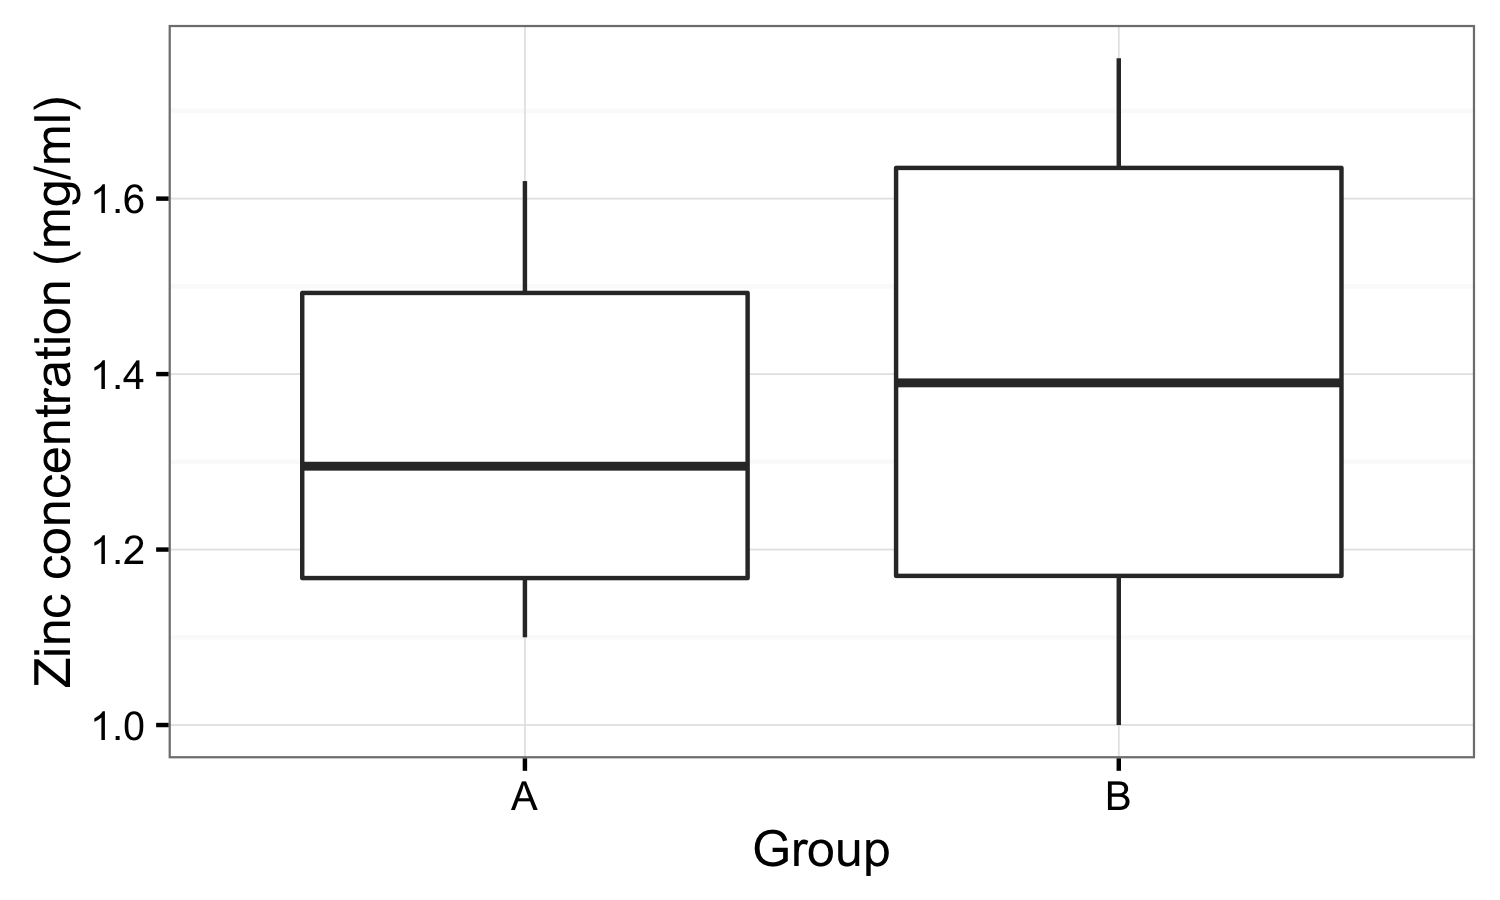
\includegraphics[width=5in]{3.png}
	\caption{Zinc concentrations (in mg/ml) in the blood for two groups of rats. Group A received a calcium supplement and Group B did not.}
	\label{fig:3}
\end{figure}




\titledquestion{Use the data from Problem 3 to answer the following questions.}

\begin{parts}

\part \textbf{Set up the null and alternative hypotheses to address the research question described.}

\begin{itemize}
\item Test statistic $t=\bar{A}-\bar{B}$, where $\bar{A}$ and $\bar{B}$ are the average Zinc concentrations in the rats of group A and B, respectively.
\item Null hypothesis: $t=0$
\item Alternative hypothesis: $t\neq0$
\end{itemize}


\part \textbf{Use 1,000 simulations to perform a randomization test for testing the hypothesis in (a). What is your p-value?}

The observed difference between sample averages is $-0.07755$, which, based on the 1,000 simulations in the randomization distribution, corresponds to a two-sided p-value of $0.261$.

\part \textbf{Draw the reference distribution of your test statistic based on 1,000 simulations.}

See Figure \ref{fig:4c}.

\begin{figure}[h!]
	\centering
	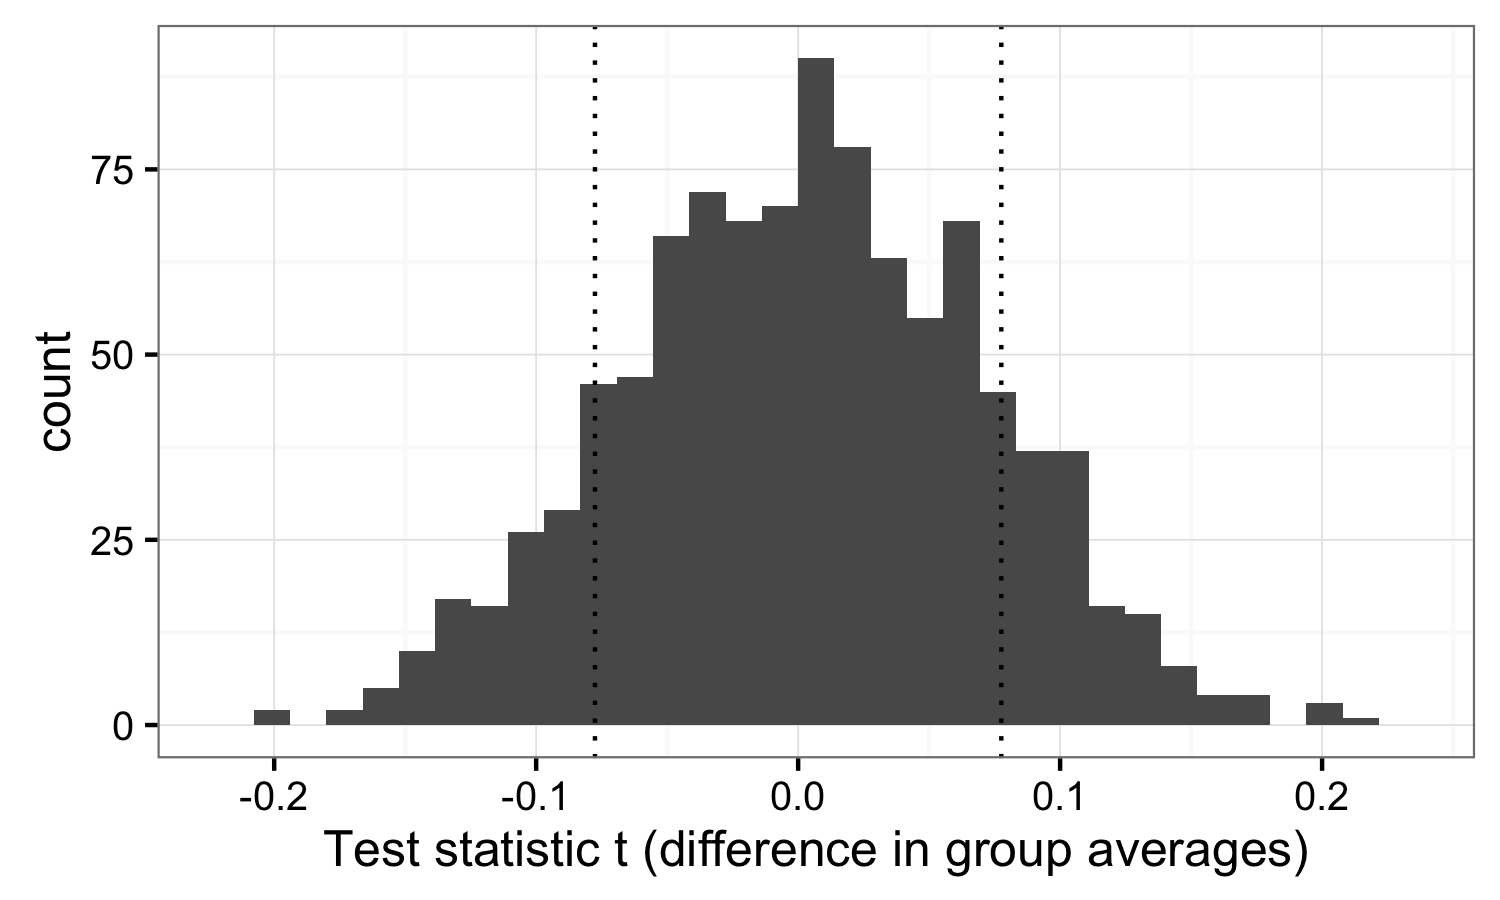
\includegraphics[width=5in]{4c.png}
	\caption{Reference distribution of $t$, based on 1,000 simulations.}
	\label{fig:4c}
\end{figure}


\part \textbf{Write a brief summary of your findings and possible recommendations for the researchers.}

The available data does not provide conclusive evidence that the calcium supplement given to group A, but not to group B, had an effect in blood Zinc concentrations. The p-value, $0.261$, associated with the test statistic indicates that there isn't enough evidence to conclusively reject the null hypothesis.



\end{parts}




\titledquestion{\ramsey 2.12}

\todo{problem 5 (2.12)}

\titledquestion{\ramsey 2.14}

Using the \texttt{t.test} R function,
\begin{code}
fishOilData <- Sleuth3::ex0112
t.test(formula=BP~Diet, data=fishOilData,
       var.equal=TRUE, conf.level=0.95)
\end{code}

a 95\% confidence interval for $\mu_2 - \mu_1$ is given by $2.225 < \mu_2 - \mu_1 < 13.203$.

Since we care about a one-sided effect (that the fish oil diet resulted in greater reduction of blood pressure), we could alternatively look at a one-sided 95\% confidence ``interval'':
\begin{code}
t.test(formula=BP~Diet, data=fishOilData,
       var.equal=TRUE, conf.level=0.95,
       alternative="greater")
\end{code}

to find $3.224 < \mu_2 - \mu_1 < \infty$.

The one-sided p-value is $0.004931$.



\titledquestion{\ramsey 2.16}

\titledquestion{\ramsey 2.23}









\end{questions}

\listoftodos

\end{document}
